\documentclass[11pt]{article}
\usepackage{geometry}                % See geometry.pdf to learn the layout options. There are lots.
\geometry{letterpaper}                   % ... or a4paper or a5paper or ... 
%\geometry{landscape}                % Activate for for rotated page geometry
%\usepackage[parfill]{parskip}    % Activate to begin paragraphs with an empty line rather than an indent
\usepackage{graphicx}
\usepackage{amssymb,amsmath}
\usepackage{epstopdf}
\usepackage{pgf}
\usepackage{pgfpages}
\usepackage{tikz}
\usetikzlibrary{arrows,backgrounds}
\usepgflibrary{shapes}
\DeclareGraphicsRule{.tif}{png}{.png}{`convert #1 `dirname #1`/`basename #1 .tif`.png}

\begin{document}

 \begin{figure}[htpb]
   \begin{center}
       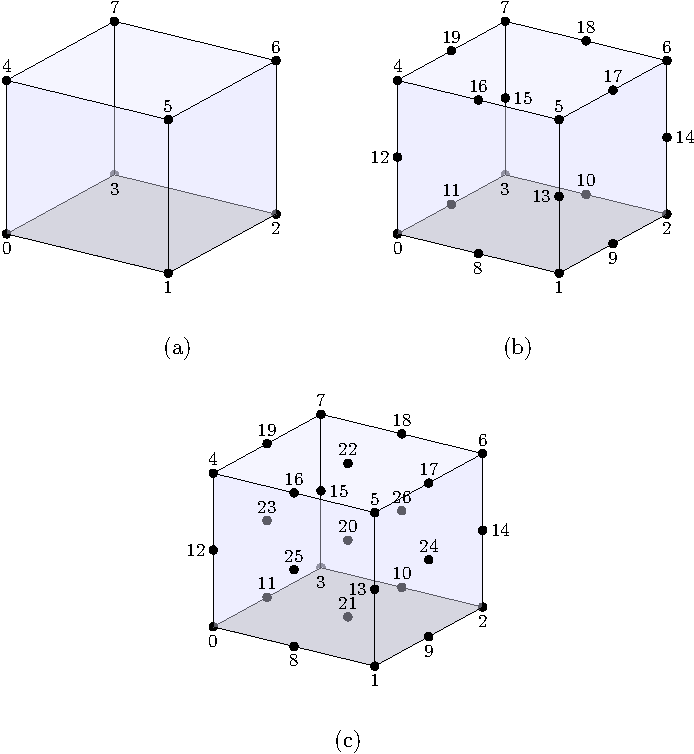
\includegraphics[width=5.0in]{hex_node.pdf}%
     \end{center}
    \begin{center}  (a) \hspace{5cm} (b) \end{center}
   \caption{(a) Base line {\tt (line<2>)} and (b) extended line {\tt (line<3>)} topology in Shards.}
  \label{fig:line}
  \end{figure}
\end{document}  
